\newpage

\subsubsection{UCA 5 - Visualizzazione dello storico accessi presso un'organizzazione}
\begin{figure}[h]
	\centering	
	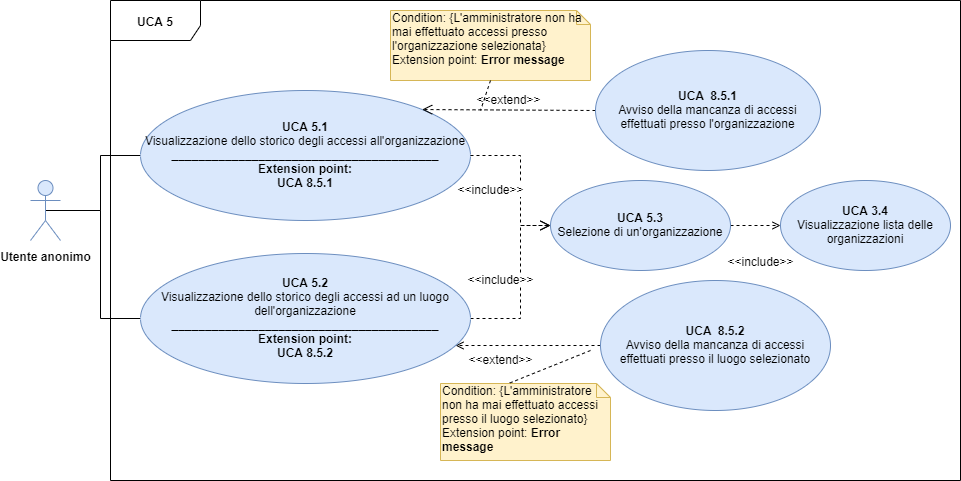
\includegraphics[scale=0.5]{sezioni/UseCase/Immagini/UCA5.png}
	\caption{UCA 5 - Visualizzazione dello storico accessi presso un'organizzazione}
\end{figure}

\begin{itemize}
    \item \textbf{Attori primari:} Utente anonimo, Utente riconosciuto
    \item \textbf{Precondizione:} L'utente ha precedentemente aggiunto l'organizzazione di cui vuole visualizzare i propri accessi alla lista delle organizzazione preferite.
    \item \textbf{Postcondizione:} L'utente visualizza la lista degli accessi effettuati presso i luoghi dell'organizzazione. Inoltre, se l'utente si trova all'interno di un luogo viene visualizzato il tempo passato lì dentro fino a quel momento.
    \item \textbf{Scenario principale:} L'utente può visualizzare la lista dei propri accessi (con nome del luogo, timestamp di ingresso, di uscita, e tempo di permanenza) presso un'organizzazione (previa selezione), se questa non è vuota, e se si trova all'interno di un luogo, visualizza il tempo passato al suo interno fino a quel momento.
    \item \textbf{Inclusioni:}
    \begin{itemize}
        \item UCA 5.1 - Visualizzazione della lista delle organizzazioni preferite;
        \item UCA 5.2 - Visualizzazione della lista degli accessi presso un'organizzazione preferita.
    \end{itemize}
\end{itemize}


\subsubsection{UCA 5.1 - Visualizzazione della lista delle organizzazioni preferite}
\begin{itemize}
    \item \textbf{Attori primari:} Utente anonimo, Utente riconosciuto
    \item \textbf{Precondizione:} L'utente ha precedentemente aggiunto le organizzazioni da visualizzare nella lista delle organizzazioni preferite.
    \item \textbf{Postcondizione:} L'utente visualizza la lista delle proprie organizzazioni preferite.
    \item \textbf{Scenario principale:} L'utente visualizza la lista delle proprie organizzazioni preferite.
    \item \textbf{Scenario alternativo:} L'utente tenta di visualizzare lo storico degli accessi ma non ha inserito alcuna organizzazione nella lista di organizzazioni preferite.
    \item \textbf{Flusso di eventi:}
    \begin{enumerate}
        \item L'utente seleziona la funzionalità dello storico degli accessi.
    \end{enumerate}
    \item \textbf{Estensioni:}
    \begin{itemize}
        \item UCA 7.5.1 - Avviso di assenza di organizzazioni preferite.
    \end{itemize}
\end{itemize}

\subsubsection{UCA 5.2 - Visualizzazione della lista degli accessi presso un'organizzazione preferita}
\begin{itemize}
    \item \textbf{Attori primari:} Utente anonimo, Utente riconosciuto
    \item \textbf{Precondizione:} L'utente ha selezionato dalla lista delle organizzazioni preferite un'organizzazione di cui visualizzare i propri accessi.
    \item \textbf{Postcondizione:} L'utente visualizza la lista degli accessi effettuati presso i luoghi dell'organizzazione. Se si trova all'interno di un luogo viene visualizzato il tempo passato lì dentro fino a quel momento.
    \item \textbf{Scenario principale:} L'utente può visualizzare tutti gli accessi da lui fatti presso i luoghi dell'organizzazione selezionata (con descrizione del luogo, timestamp di ingresso, di uscita, e tempo di permanenza), in modalità di tracciamento anonimo e autenticato (se disponibile).
    \item \textbf{Scenario alternativo 1:} L'utente ha effettuato l'accesso presso il luogo dell'organizzazione ma non ne è ancora uscito. In questo caso, viene visualizzato un timer con il tempo trascorso dal momento in cui è entrato.
    Una volta uscito dal luogo, vale il comportamento descritto nello scenario principale.
    \item \textbf{Scenario alternativo 2:} L'utente 
    \item \textbf{Flusso di eventi:}
    \begin{enumerate}
        \item UCA 5.1.
    \end{enumerate}
    \item \textbf{Estensioni:}
    \begin{itemize}
        \item UCA 7.5.2;
        % non sempre li eseguo, solo se l'utente lo chiede
        \item UCA 5.2.2;
        \item UCA 5.2.3;
        \item UCA 5.2.4.
    \end{itemize}
\end{itemize}

\subsubsection{UCA 5.2.2 - Ordinamento per data decrescente della lista degli accessi}
\begin{itemize}
    \item \textbf{Attori primari:} Utente anonimo, Utente riconosciuto
    \item \textbf{Precondizione:} L'utente ha a disposizione una lista di accessi presso uno o più luoghi di un organizzazione preferita.
    \item \textbf{Postcondizione:} L'utente ottiene la lista di accessi iniziale riordinata in ordine decrescente.
\end{itemize}

\subsubsection{UCA 5.2.3 - Ordinamento per data crescente della lista degli accessi}
\begin{itemize}
    \item \textbf{Attori primari:} Utente anonimo, Utente riconosciuto
    \item \textbf{Precondizione:} L'utente ha a disposizione una lista di accessi presso uno o più luoghi di un organizzazione preferita;
    \item \textbf{Postcondizione:} L'utente ottiene la lista di accessi iniziale riordinata in ordine crescente (ovvero una data meno recente è considerata più piccola di una data più recente).
\end{itemize}

\subsubsection{UCA 5.2.4 - Filtro per luogo della lista degli accessi presso un'organizzazione prferita}
\begin{itemize}
    \item \textbf{Attori primari:} Utente anonimo, Utente riconosciuto
    \item \textbf{Precondizione:} L'utente ha a disposizione una lista di accessi presso uno o più luoghi di un organizzazione preferita.
    \item \textbf{Precondizione:} L'utente ottiene la lista di accessi iniziale presso un singolo luogo selezionato.
\end{itemize}